% Metódy inžinierskej práce

\documentclass[10pt,twoside,slovak,a4paper]{coursepaper}

\usepackage[slovak]{babel}
%\usepackage[T1]{fontenc}
\usepackage[IL2]{fontenc} % lepšia sadzba písmena Ľ než v T1
\usepackage[utf8]{inputenc}
\usepackage{graphicx}
\usepackage{url} % príkaz \url na formátovanie URL
\usepackage{hyperref} % odkazy v texte budú aktívne (pri niektorých triedach dokumentov spôsobuje posun textu)

\usepackage{cite}
%\usepackage{times}

\pagestyle{headings}

\title{Implementácia a využívanie modelov počítačoveho videnia v praxi \thanks{Semestrálny projekt v predmete Metódy inžinierskej práce, ak. rok 2020/21, vedenie: Vladimír Mlynarovič}} % meno a priezvisko vyučujúceho na cvičeniach

\author{Ján Mareček\\[2pt]
	{\small Slovenská technická univerzita v Bratislave}\\
	{\small Fakulta informatiky a informačných technológií}\\
	{\small \texttt{xmarecek@stuba.sk}}
	}

\date{\small 3. november 2021} % upravte



\begin{document}
\maketitle


\begin{abstract}
Odborný článok na tému "Implementácia a využívanie modelov Počítačoveho videnia v praxi " pozostáva z 4 kapitol. Prvá kapitola je venovaná používaniu počítačoveho videnia s využitím programovacích jazykov ako Python a C++ a knižnice OpenCV.Druhá kapitola je venovaná druhom a trénovaniu modelov počítačoveho videnia.Tretia kapitola je venovaná výhodam a nevýhodám počítačoveho videnia. Obsahom štvrtej kapitoli je využitie počítačoveho videnia v praxi. 
\end{abstract}

\section{Počítačové videnie}
Počítačové videnie je automatizovaná extrakcia informácií z obrázkov.Informáciu može predstavovať hocičo od 3D modelov,videa alebo obrázka.Niekedy sa počítačové videnie snaží napodobňovať ľudské videnie, inokedy využíva dáta alebo štatistiky.Praktické počítačove videnie je mix programovania,modelovania a matematiky.Matematická časť pomáha pochopiť špecifické algoritmy,k toré sú používané.

\section{Programovacie jazyky a knižnice počítačoveho videnia}


Jeden z najpopularnejších, ak nie najpopularnejší programovací jazyk pre prácu s počítačovým videním je Python.Python je interpetovaný,interaktívny programovací jazyk s dobrou podporou na spracovávanie obrazu.Od verzie 2.6 máme pri práci s Pythonom k dispozícii väčšinu balíkov, ktoré pri práci potrebujeme. Od verzie 3.x.x si zmenila syntax pre ale kompatibilita s balíkmi pre počítačové videnie ostala rovnaká.\cite{Python-CV}


NumPy je knižnica pre programovací jazyk Python .Je užitočná na prácu s vektormi,  maticami a ich operáciami na vysokej úrovni ,ktoré sú potrebné na fungovanie počítačoveho videnia.Dané typy su reprezentované pomocou polí.


V počítačovom videní sa stretneme aj s inými knižnicami jazyka Python .Knižnica Matplotlib je využivaná pre vizualizáciu  výsledkov.Knižnica SciPy je využivaná keď potrebujeme využivať pokročilejšie matematické funkcie alebo algoritmy.\cite{Python-CV}

%\subsection{Počitačové videnie a C++} \label{ina:nejake}
%C++ je v dnešnej dobe taktiež veľmi populárny pre prácu s počitačovým videním .

OpenCV je  open-source knižnica napísaná v C++ ,ktorá obsahuje algoritmy a funkcie zamerané na počítačové videnie.Najčastejšie sa používa s programovacimi jazykmi Python,C a C++ ,ale v novších verziach už bola vydaná podpora aj na JavaScript. Má modulárnu štruktúru čo znamená, že obsahuje niekoľko hlavných knižníc.
\begin{itemize}
\item Hlavné knižnice OpenCv sa zaraďujú napríklad:
	\begin{enumerate}
	\item Image Processing-modul na spracovávanie obrázkov
	\item Video Analysis-modul na spracovávanie videí
	\item Core functionality-modul definujúci základné dátové štruktúry a funkcie ,ktoré využivajú ostatné moduly
	\item Object Detection-detekcia objektov a inštancie preddefinovaných tried (napr. tvár, oči, ľudia, autá…)
	\item High-level GUI – ľahko použiteľné rozhranie na jednoduché UI funkcie.
	\item Camera Calibration and 3D Reconstruction  – kalibrácia kamery, odhad polohy objektu, 3D rekonštrukcia.
	\item \ldots{}\cite{OpenCV}

	\end{enumerate}
\end{itemize}

\section{Modely a ich trénovanie} \label{nejaka}

\subsection{Typy modelov} \label{ina:nejako}
Rôzne typy modelov nám pomáhajú riešiť rôzne typy problémov.Aké predmety sú na obrázku? Kde sú predmety na obrázku?

 Klasifikácia obrázkov: Snaží sa identifikovať najvýznamnejšiu triedu objektu.Triedu môžme chápať ako označenie,napr. pri identifikácií topánok(bežecká obuv,...)

Detekcia objektov: Používa sa, keď je doležitá poloha objektu.Vracia množstvo súradníc nazývaných ohraničujúci rámček.Príklad takéhoto modelu može byť model na detekciu osôb(AlwaysAI/mobilenet).

Segmentácia obrazu: Keď je dôležitý presný tvar objektu využijeme segmentáciu obrazu.Pre presnú segmentáciu klasifikuje každý pixel.

 Detekcia orientačných bodov: Využíva sa na určenie dôležitých bodov,ktoré zachytávajú dôležite prvky objektu.Môžme použiť model na odhad pózy(AlwaysAl/human-pose).
\cite{CV-framework}


\subsection{Typy údajov pre školenie počítačového videnia a ich trénovanie}
Generovanie množiny údajov:Na učenie modelu počítačového videnia potrebujeme kvalitné údaje.Za kvalitný údaj sa považuje ten, čo je podobný údajom z reálneho sveta,ktoré budú použité na trénovanie modelu.


Typy generovania množín údajov: Podľa toho, či chceme nech model vykonáva jednu konkrétnu úlohu alebo chceme všeobecný model, potrebujeme aj rôzne typy údajov.
Ak chceme konktrétny model budeme potrebovať na jeho tréning špecifické dáta a obrázky, ktoré sú čo najviac podobné danej špecifikácii.
Použitie existujúcej anotovanej množiny údajov: Výrazne môžu skrátiť čas potrebný na trénovanie modelu ale zároveň nemáme takú kontrolu nad kvalitou údajov.Populárne verejné súbory údajov sú napr. PASCAL Visual Object Classes (VOC),ImageNet,...
Použitie vlastných údajov : vlastný súbor údajov tvorený z voľne dostupných videí a obrázkov online.Na rozdiel od existujúcej anotovanej množiny ich treba anotovať pred použitím. Použitie digitálne generovaného súboru:Používa sa, ak nie sme sami schopní zhromaždiť dostatok údajov.Vedie k lepšiemu výkonu.
\cite{CV-framework}

Zhromaždené a anotované údaje sa použijú ako vstup pre tréning modelu.Prechádzajú a porovnavajú sa údaje, až kým nedosiahneme dobrý výkon, na základe špecifikácií pre každý typ modelu.


Transfer Learning: Využíva poznatky zo všeobecného tréningu a aplikuje ich na iné špecifickejšie možnosti.
Testovacia aplikácia: Po vytvorení modelu na ňom otestujeme aj nové údaje, a zistíme či model reaguje a pracuje ako očakávame.Nejde o automatizovaný test, ale jeho výhoda je, že umožňuje rýchlo identifikovať nedostatky alebo prípady, kedy model nefunguje spoľahlivo.Potom na model použijeme situácie prípadov, kedy nefungoval úplne správne a opravíme to.\cite{CV-framework}
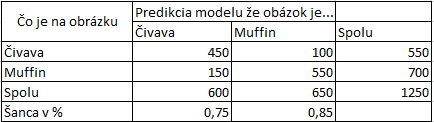
\includegraphics[scale=1]{tabulka.png}
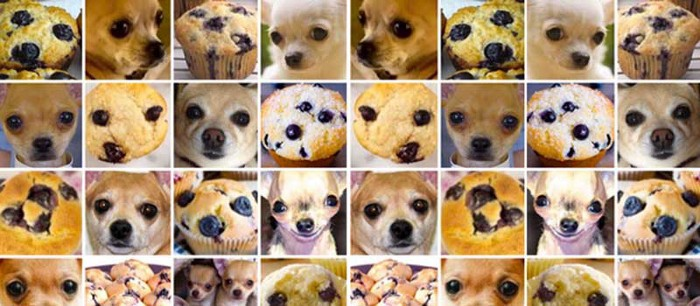
\includegraphics[scale=0.5]{civava_vs_muffin.jpeg}
\cite{Conditional-Probability}
\centering
%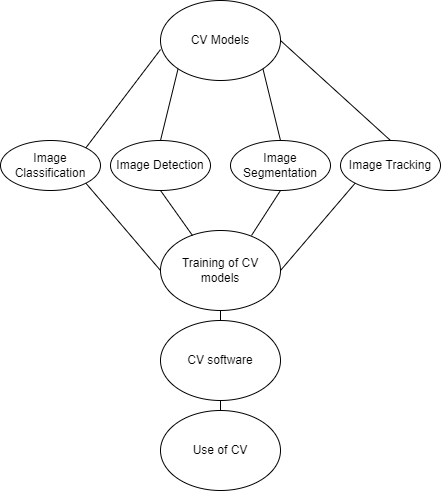
\includegraphics[scale=1.0]{diagram.pdf}




\section{Výhody a nevýhody počítačového videnia} \label{ina}
Ako každá iná technologia aj počítačové videnie má svoje výhody a nevýhody.
\begin{itemize}
\item Porovnanie s ľudským videním
	\begin{itemize}
	\item ľudské videnie: zdroj obrazu → oko → kognitívny systém
	\item počítačové videnie: zdroj obrazu → kamera → počítač
	\end{itemize}
\end{itemize}

\begin{itemize}
\item Výhody
	\begin{enumerate}
	\item Uľahčuje množstvo procesov
	\item Úplné frekvenčné spekrum pre získanie obrazov
	\item Jednoduchý a rýchly spôsob získavania údajov
	\item Generovanie presných a presných údajov
	\item Finančne efektívne
	\end{enumerate}
\end{itemize}

\begin{itemize}
\item Nevýhody
	\begin{enumerate}
	\item Treba spracovávať veľmi veľké množstvo informácií
	\item Citlivé na osvetlenie a rôzne iné javy
	\item Reálny svet transformujeme 3D na 2D
	\item Je potrebné veľké množstvo pamäte
	\item Veľké množstvo nadbytočných údajov 
	\cite{CV-inspection-system}
	\end{enumerate}
\end{itemize}

\section{Využitie počítačového videnia}
Počitačové videnie sa dnes využíva v každom odvetvý informačných technológii na svete. Jeho najväčšie využitie je v priemysle kde dokáže efektívne kontrolovať kvalitu produktov , alebo v zdravotníctve kde zachraňuje množstvo životou kontrolou a identifikáciou problémov. Využitie má aj v rekreacií kde slúži ako zábava pre programátorov alebo nadšendov drovo , ktoré sú často využívané pri amatérkej práci s počitačovým videním . \cite{CV-inspection-system} 
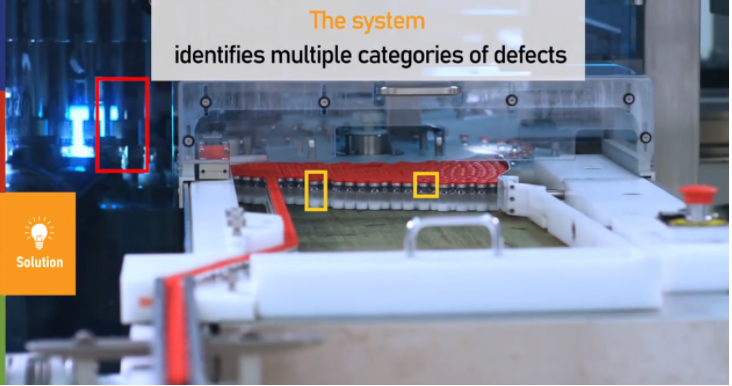
\includegraphics[scale=0.75]{defect_detection.png}
\cite{inspection-in-manufacturing}
\section{Záver} \label{zaver} % prípadne iný variant názvu



%\acknowledgement{Ak niekomu chcete poďakovať\ldots}


% týmto sa generuje zoznam literatúry z obsahu súboru literatura.bib podľa toho, na čo sa v článku odkazujete
\bibliography{literatura}
\bibliographystyle{alpha} % prípadne alpha, abbrv alebo hociktorý iný
\end{document}
